\chapter{Results and Analysis} \label{Chap4}

\section{Final Model}

\subsection{Success rate on Baseline codes}
The final model described in the methods section uses the evolutionary search algorithm as the main structure with implementations of elitism, tournaments selection and adaptive mutation rates. Through extensive testing on smaller codes namely the \([[5,1,3]]\) and \([[7,1,3]]\) codes we were able to fine tune parameters that scale moderately well with larger code sizes. In Figure \ref{fig:Final model success rate} below, we show the average success rate of the search algorithm at finding the minimum 2-qubit transvection implementations of the logical H and S operators on the \([[5,1,3]]\) and \([[7,1,3]]\) codes.

\begin{figure}[H]
    \centering
    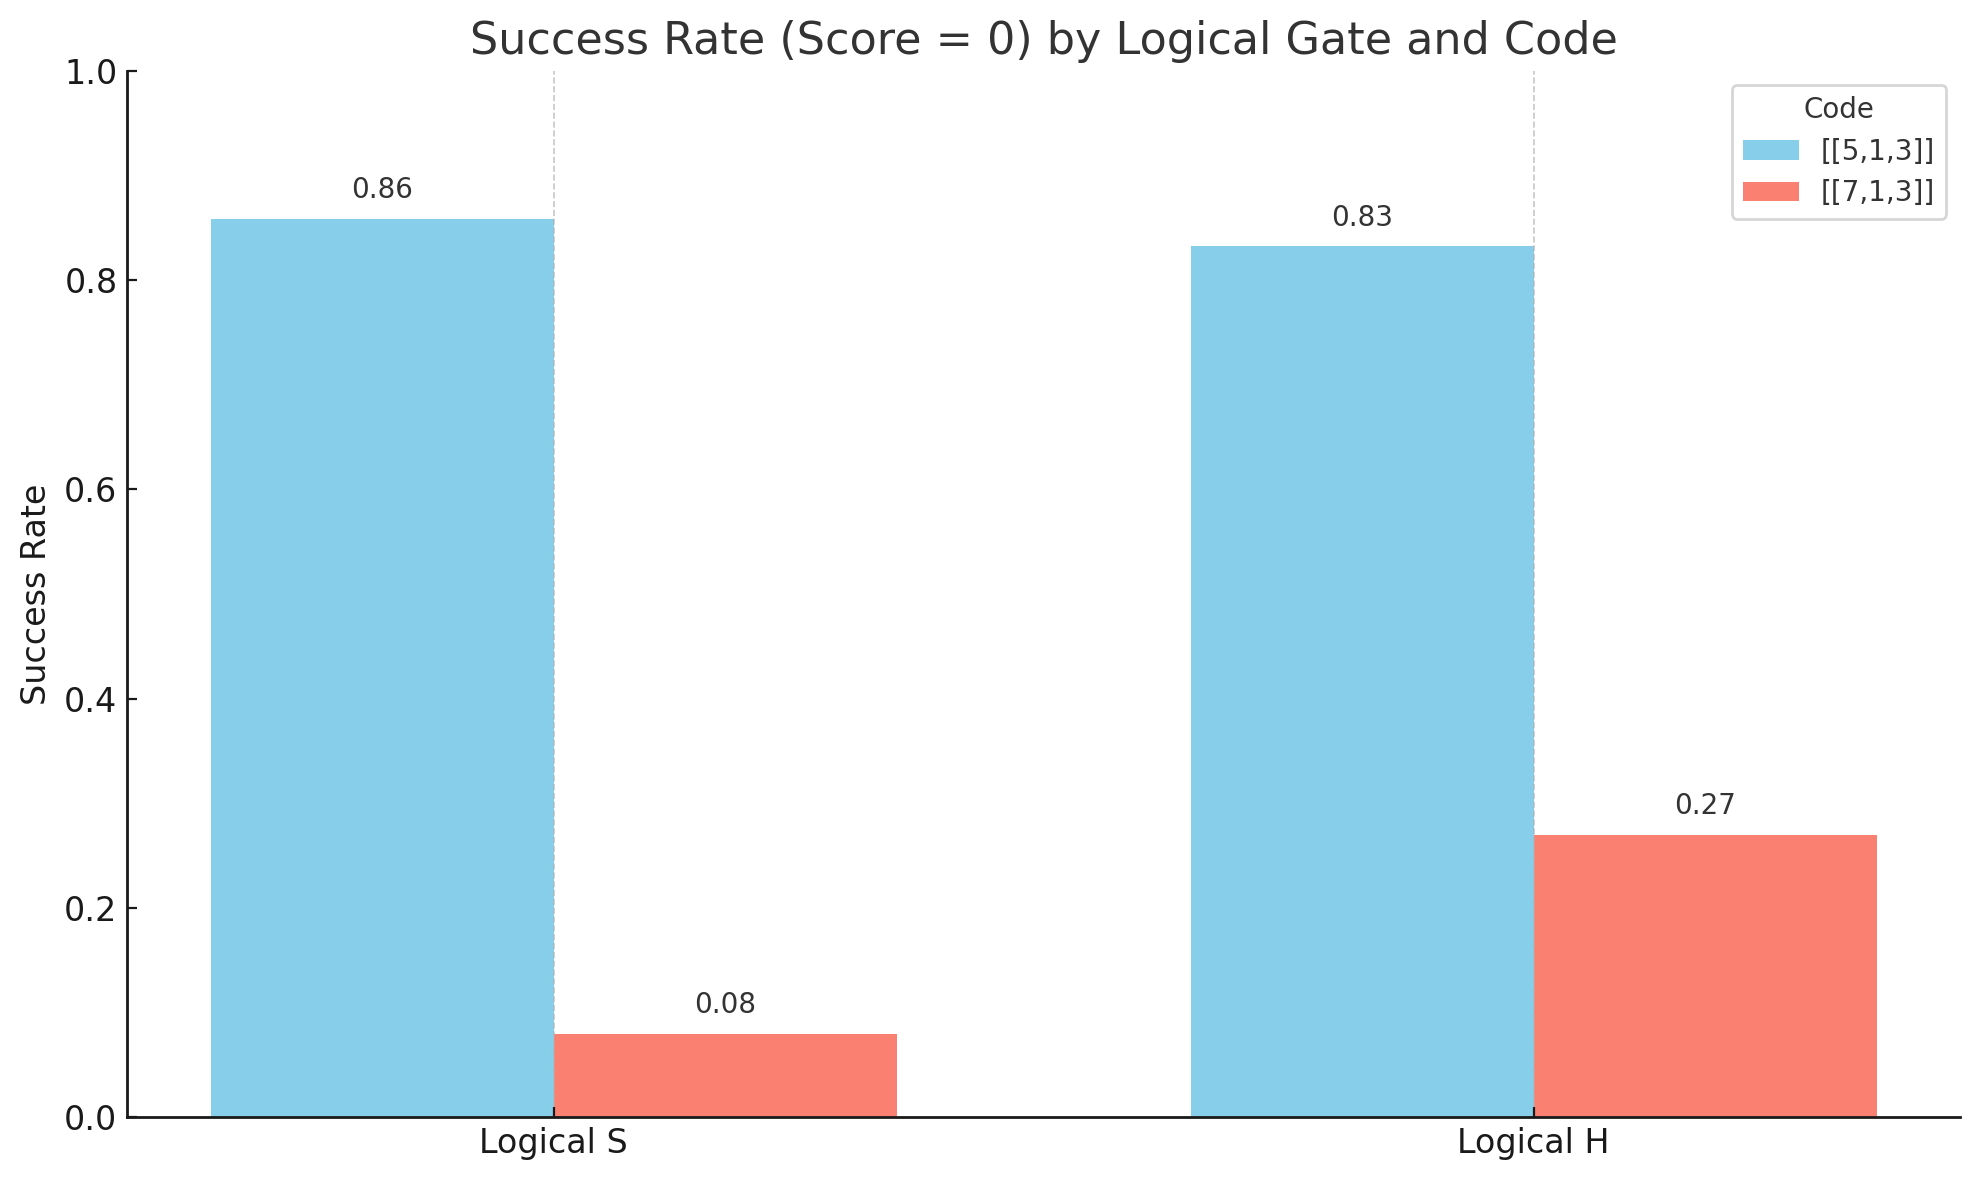
\includegraphics[width=1\linewidth]{Logos/output-6.png}
    \caption{Individual success rate of populations in the search algorithm for logical \(S\) and \(H\) in the [[5,1,3]] and [[7,1,3]] codes. number of runs: \((S,5)=500\), \((S,7)=88\), \((S,5)=1000\), \((S,5)=100\).}
    \label{fig:Final model success rate}
\end{figure}

Figure \ref{fig:Final model success rate} clearly illustrates the sharp decline in success rate when transitioning from the [[5,1,3]] code to the [[7,1,3]] code. This dramatic drop aligns with expectations when considering the exponential growth in search space. According to Equation \ref{eq:number of possible logical cliffords}, the [[5,1,3]] code yields a search space of approximately 5.28 billion possible implementations, whereas the [[7,1,3]] code expands this to an overwhelming \(1.73\times 10^{20}\), a difference of over 32.7 billion times. Given this massive increase, a corresponding decrease in the success rate of individual runs is anticipated.

In larger search spaces, not only is it harder to locate optimal solutions, but the likelihood of encountering numerous local minima also increases. Evidence of this can be found in Table \ref{tab:frequancy table of scores}, which shows that for the [[5,1,3]] code, the algorithm frequently converges to suboptimal scores of 2 and 4. This suggests the presence of at least two dominant local minima. In the case of the [[7,1,3]] code, the distribution of scores implies the presence of seven or more local minima, assuming these plateaus result from the algorithm becoming trapped, rather than from slow convergence. 

\begin{table}[h!]
\centering
\caption{Frequency of Scores (excluding 0) for logical \(H\)}
\label{tab:frequancy table of scores}
\begin{tabular}{ccc}
\toprule
\textbf{Score} & \textbf{[[5,1,3]]} & \textbf{[[7,1,3]]} \\
\midrule
2 & 96 & 6 \\
4 & 72 & 10 \\
6 & 0 & 15 \\
8 & 0 & 22 \\
10 & 0 & 16 \\
12 & 0 & 3 \\
14 & 0 & 1 \\
\bottomrule
\end{tabular}
\end{table}

\subsection{Model Execution times}
One last point to mention is the code runtime. For the [[5,1,3]] code we achieved a relatively short average execution time of \(135\pm 70\) seconds and the for the [[7,1,3]] this average time was \(4300\pm 600\) seconds. Similarly to before the this increase is expected as the search space increases drastically from [[5,1,1]] to [[7,1,3]]. A point to note is that the average runtime is approximately halved when the algorithm is executed serially rather than in parallel. This somewhat counterintuitive result is likely due to the behavior of Python's Just-In-Time (JIT) compiler, which may not optimize as effectively when using multiprocessing with a pool of worker processes. Despite this, running the algorithm in parallel remains the preferred approach. Even with a modest setup of 8 CPU cores, parallel execution effectively doubles the throughput compared to the serial version, allowing for significantly more runs to be completed in the same amount of time.

\section{Exploring implementations of the Toric Code}

\begin{figure}[h]
    \centering
    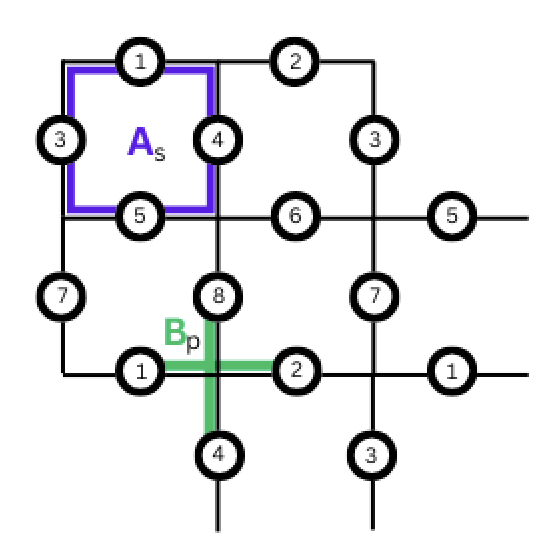
\includegraphics[width=0.5\linewidth]{Logos/Screenshot 2025-04-01 at 13.41.28.png}
    \caption{Repeating structure of the \([[8,2,2]]\) Toric code}
    \label{fig:[[8,2,2]] Toric code}
\end{figure}

The Toric code is a well known example of a topological stabiliser code (see Appendix \ref{Appendix C} that encodes quantum information into the global properties of a two-dimensional spin lattice. Its topological nature provides intrinsic protection against local errors, as logical qubits are stored non-locally across the lattice, making it particularly attractive for fault-tolerant quantum computing. Additionally, the Toric code's regular structure and compatibility with nearest-neighbour interactions make it well-suited for implementation on two-dimensional quantum hardware architectures. Here we have tested the algorithm on the \([[8,2,2]]\) Toric code to find low depth implementations logical \(S\), \(H\), \(CZ\), and \(CNOT\) (see Appendix \ref{Appendix D} for matrix representation of the Logical operators). These gates are not enough to perform universal computation however they do serve as a good showcase for the potential of our algorithm. Clifford gates are a foundational component of fault-tolerant quantum computing, especially in stabiliser code frameworks, and are often used in conjunction with magic state distillation to achieve universality. Efficient implementations of these logical operations are essential for reducing circuit depth, lowering error propagation, and improving overall computational fidelity.

\subsection{Logical S, H, CZ, and CNOT}
Using the algorithm, we were able to find an implementation of the logical \(\bar{S}\) gate consisting solely of single-qubit Clifford operations, meaning zero two-qubit transvections and, perhaps more surprisingly, no SWAP operations either. The resulting logical operator can be expressed as:

\begin{equation}
    \bar{S} = SIIIISII
\end{equation}

This compact form not only maintains full logical equivalence with the intended \(S\) gate on the encoded qubit, but also highlights how Clifford operations can sometimes be realised through entirely local, low-depth transformations when the structure of the code is properly leveraged. Such efficient representations are especially valuable in near-term devices, where circuit depth and entangling gates are limited by noise and hardware constraints.

For the logical H operator we also found a relatively low depth implementation consisting of a single 2-qubit transvection, some SWAPs and single-qubit Cifford layer;

Transvection \(T_v\):
\begin{equation}
    v_1 = Y_3X_7
\end{equation}

SWAPs:
\[
\begin{array}{cccccccc}
1 & 2 & 3 & 4 & 5 & 6 & 7 & 8 \\
\downarrow & \downarrow & \downarrow & \downarrow & \downarrow & \downarrow & \downarrow & \downarrow \\
2 & 6 & 3 & 4 & 1 & 5 & 7 & 8
\end{array}
\]

Single-qubit Cliffords:
\[
\begin{array}{ccccccccc}
qubit: & 1 & 2 & 3 & 4 & 5 & 6 & 7 & 8 \\
gate: & H & H & Y & HSH & H & H & Y & HSH
\end{array}
\]

For the logical CZ operator we can implement it as follows:

Transvections \(T_v\):
\begin{equation}
    v_1 = Y_1Z_4, \quad v_2=Y_2Z_4, \quad v_3=Z_3Y_5, \quad v_4=Z_3Y_6
\end{equation}

SWAPs:
\[
\begin{array}{cccccccc}
1 & 2 & 3 & 4 & 5 & 6 & 7 & 8 \\
\downarrow & \downarrow & \downarrow & \downarrow & \downarrow & \downarrow & \downarrow & \downarrow \\
1 & 2 & 3 & 8 & 5 & 6 & 7 & 4
\end{array}
\]

Single-qubit Cliffords:
\[
\begin{array}{ccccccccc}
qubit: & 1 & 2 & 3 & 4 & 5 & 6 & 7 & 8 \\
gate: & HS & HS & I & I & HS & HS & I & I
\end{array}
\]

And finally we can implement the CNOT as:

Transvections \(T_v\):
\begin{equation}
    v_1 = Z_3X_6, \quad v_2=X_1Z_8, \quad v_3=X_2Z_4, \quad v_4=Z_5X_7
\end{equation}

SWAPs:
\[
\begin{array}{cccccccc}
1 & 2 & 3 & 4 & 5 & 6 & 7 & 8 \\
\downarrow & \downarrow & \downarrow & \downarrow & \downarrow & \downarrow & \downarrow & \downarrow \\
6 & 1 & 4 & 3 & 2 & 7 & 8 & 5
\end{array}
\]

Single-qubit Cliffords:
\[
\begin{array}{ccccccccc}
qubit: & 1 & 2 & 3 & 4 & 5 & 6 & 7 & 8 \\
gate: & HSH & HSH & HS & S & HSH & HSH & HS & S
\end{array}
\]

Each implementation was verified to commute with the stabiliser group of the \([[8,2,2]] \) Toric code and to act on the logical subspace according to the expected transformation whilst preserving the stabiliser group. This ensures that all operators are indeed valid logical gates and preserve code space integrity.

It is important to note, however, that while the \(\bar{S}\) gate admits a particularly efficient implementation, not every logical Clifford operator will have a representation that avoids all two-qubit transvections. Moreover, the implementations of \(\bar{H},\space \bar{CZ}\) and \(\bar{CNOT}\) shown here may not represent the absolute optimal decompositions. For each of these gates, the algorithm was run between 24 and 32 times. Given that the 
\([[8,2,2]]\) Toric code has a significantly larger search space than smaller codes such as \([[5,1,3]]\) and \([[7,1,3]]\), it is likely that over 100 runs would be required to reliably discover the most efficient implementations.

